\section{Background}\label{Background}

\subsection{Named Routing}

Communication in NDN~\cite{ndn} is driven by receivers i.e., data consumers, through the exchange of two types of packets: Interest and Data. Both types of packets carry a name that identifies a piece of data that can be transmitted in one Data packet (see Fig.\ref{fig:ndn}).

\begin{figure}
\centering
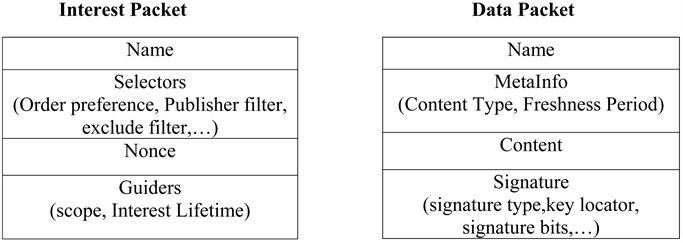
\includegraphics[height=3cm, width=8cm]{figs/ndn_packet.png}
\caption{\label{fig:ndn}NDN packets~\cite{ndn}}
\end{figure}
 
\begin{figure}
\centering
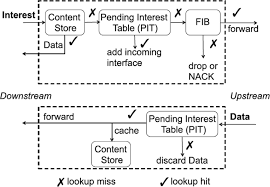
\includegraphics[height=3cm, width=8cm]{figs/process2.png}
\caption{\label{fig:process2}Forwarding Process at an NDN Node~\cite{ndn}}
\end{figure}

To carry out the Interest and Data packet forwarding functions, each NDN forwarder ~\cite{ndn} maintains three data structures: a Pending Interest Table (PIT), a Forwarding Information Base (FIB), and a Content Store (CS) (see Fig.\ref{fig:process2}), as well as a Forwarding Strategy module that determines whether, when and where to forward each Interest packet. The PIT stores all the Interests that a router has forwarded but not satisfied yet. The Content Store is a temporary cache of Data packets the router has received. The forwarding information base (FIB) table use the names to route a request to next hop routers that are closer to the data provider by performing longest-prefix matching. The hierarchy also allows name resolution and data routing information to be gathered across similar data source names, which is the key point to enhance scalability and flexibility of the network architecture. 

NLSR ~\cite{hoque2013nlsr} is a routing protocol in NDN that populates NDN’s Routing Information Base. The main design goal of NLSR is to provide a routing protocol to populate NDN’s FIB. NLSR calculates the routing table using link-state or hyperbolic routing